\section{Understanding Data Geometry}\label{data_geometry}

The initial step was to explore the geometry of the data. The \emph{Fashion-MNIST} dataset comprises 70,000 grayscale images 
(60,000 for training and 10,000 for testing) of clothing items, divided into 10 categories. Each image is 28x28 pixels, 
resulting into 784 features per image. Given this high dimensionality, I explored several dimensionality reduction methods to gain 
a qualitative and visual understanding of the data structure. I began with classical Principal Component Analysis (PCA) and then 
proceeded to kernel PCA, experimenting with both polynomial and gaussian kernels to capture more complex patterns and non-linear
structures within the data. Performing kernel PCA on the entire dataset proved to be computationally demanding even within the cluster environment, 
particularly in terms of memory usage. To address this, I selected a reduced training set consisting of 7,500 datapoints (1/8 of the 
original training set size). Before proceeding with any further analysis, I ensured that this subset was representative of all the classes, 
maintaining a balanced distribution across the categories, as shown in \Cref{fig:dataset_representativeness}.

\begin{figure}[ht]
    \centering
    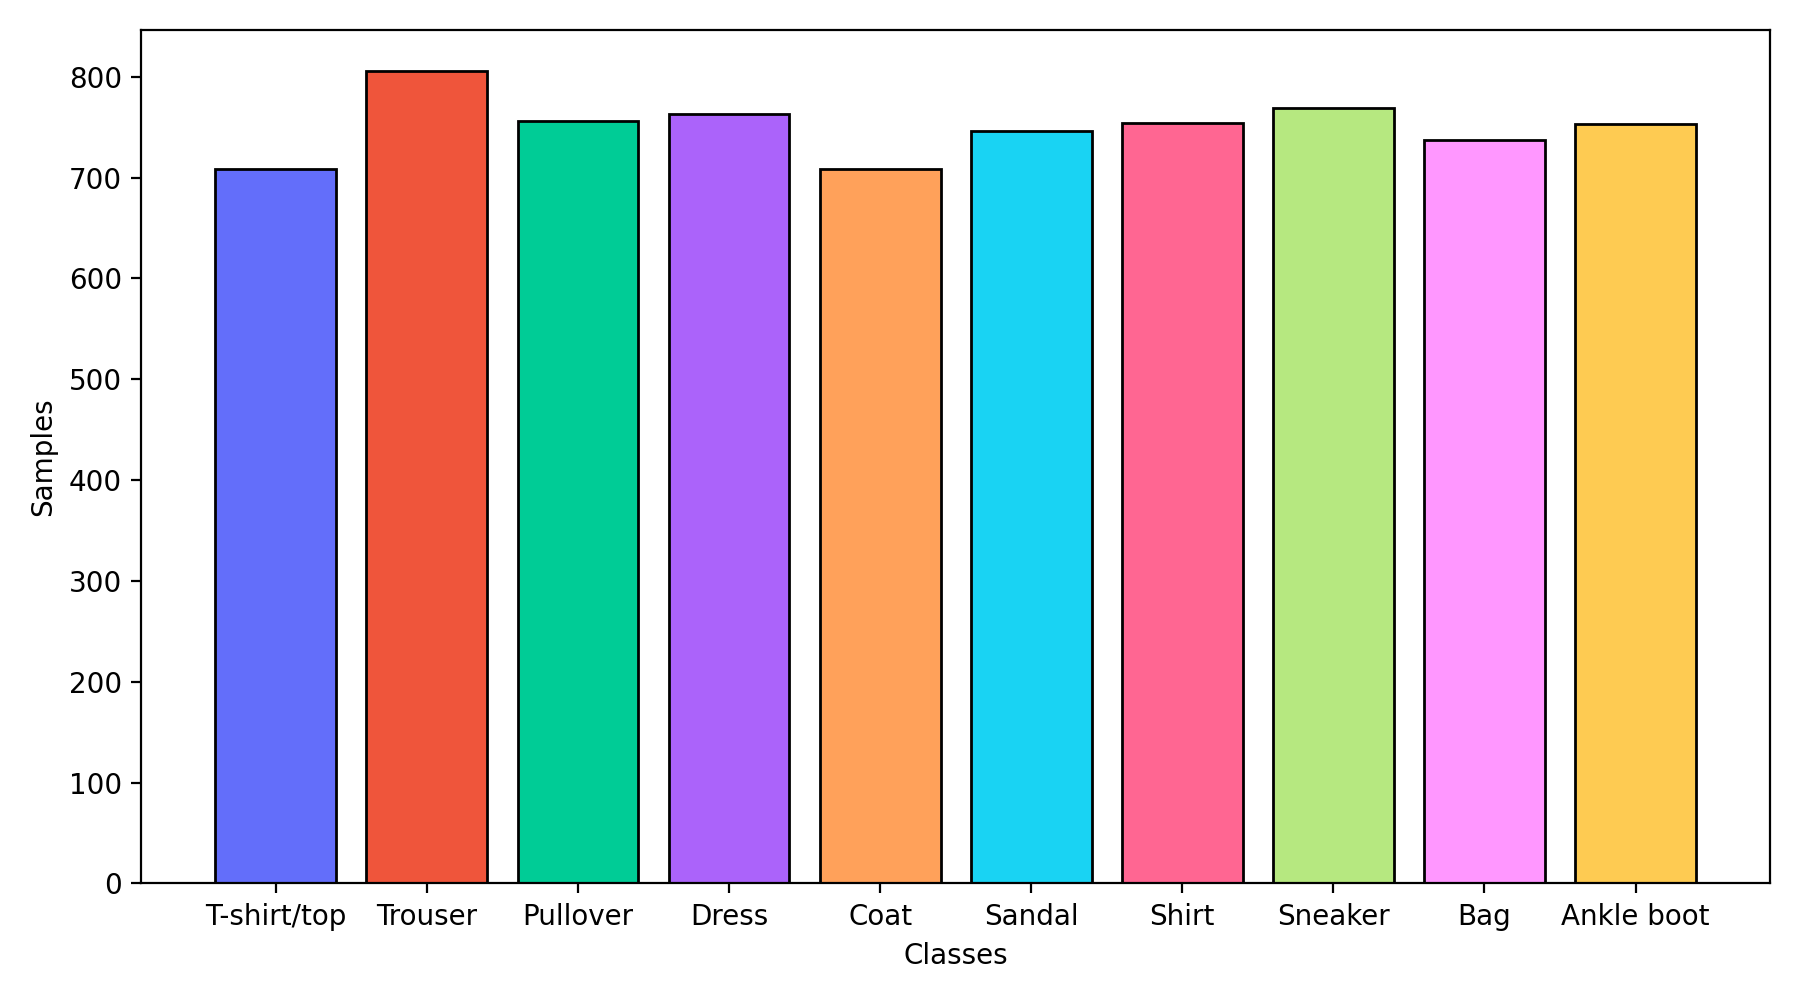
\includegraphics[width=0.65\textwidth]{../plots/reduced_dataset_representativeness.png}
    \caption{\footnotesize Distribution of the reduced training set across the 10 classes.}
    \label{fig:dataset_representativeness}
\end{figure}
\newpage
Once obtained the reduced dataset, I applied some pre-processing transformations. Instead of applying Z-normalization to the data 
on their original scale $(0-255)$, I scaled the pixel values by dividing them by $255$. This scaling step maps the pixel 
values into a more compact range of [0, 1], which is indeed a general good practice for feeding ML models. After scaling, I 
proceeded with centering the data, which is an essential prerequisite for applying PCA. However, I avoided dividing by the standard 
deviation to prevents issues where low standard deviation in pixels (\emph{e.g., corners}) could cause their values to explode.\\[0.2cm]
After completing the data preparation phase, I moved to dimensionality reduction. To explore the impact of different 
configurations I performed a tuning phase, testing various values for \texttt{gamma} (scale parameter for gaussian kernel PCA)
and \texttt{deg} (degree for polynomial kernel PCA). More in details, I tested \texttt{gamma} $\in \{0.001,0.005,0.01,0.05,0.1,0.5,1,5\}$ and
\texttt{deg} $\in \{2,3,4,5\}$. Below I present only the most interesting outcomes from this stage, but for all those 
interested in further details, please refer to the project repository, where all the plots generated during this process are available.

\begin{figure}[!htb]
    \begin{minipage}{0.5\textwidth}
      \centering
      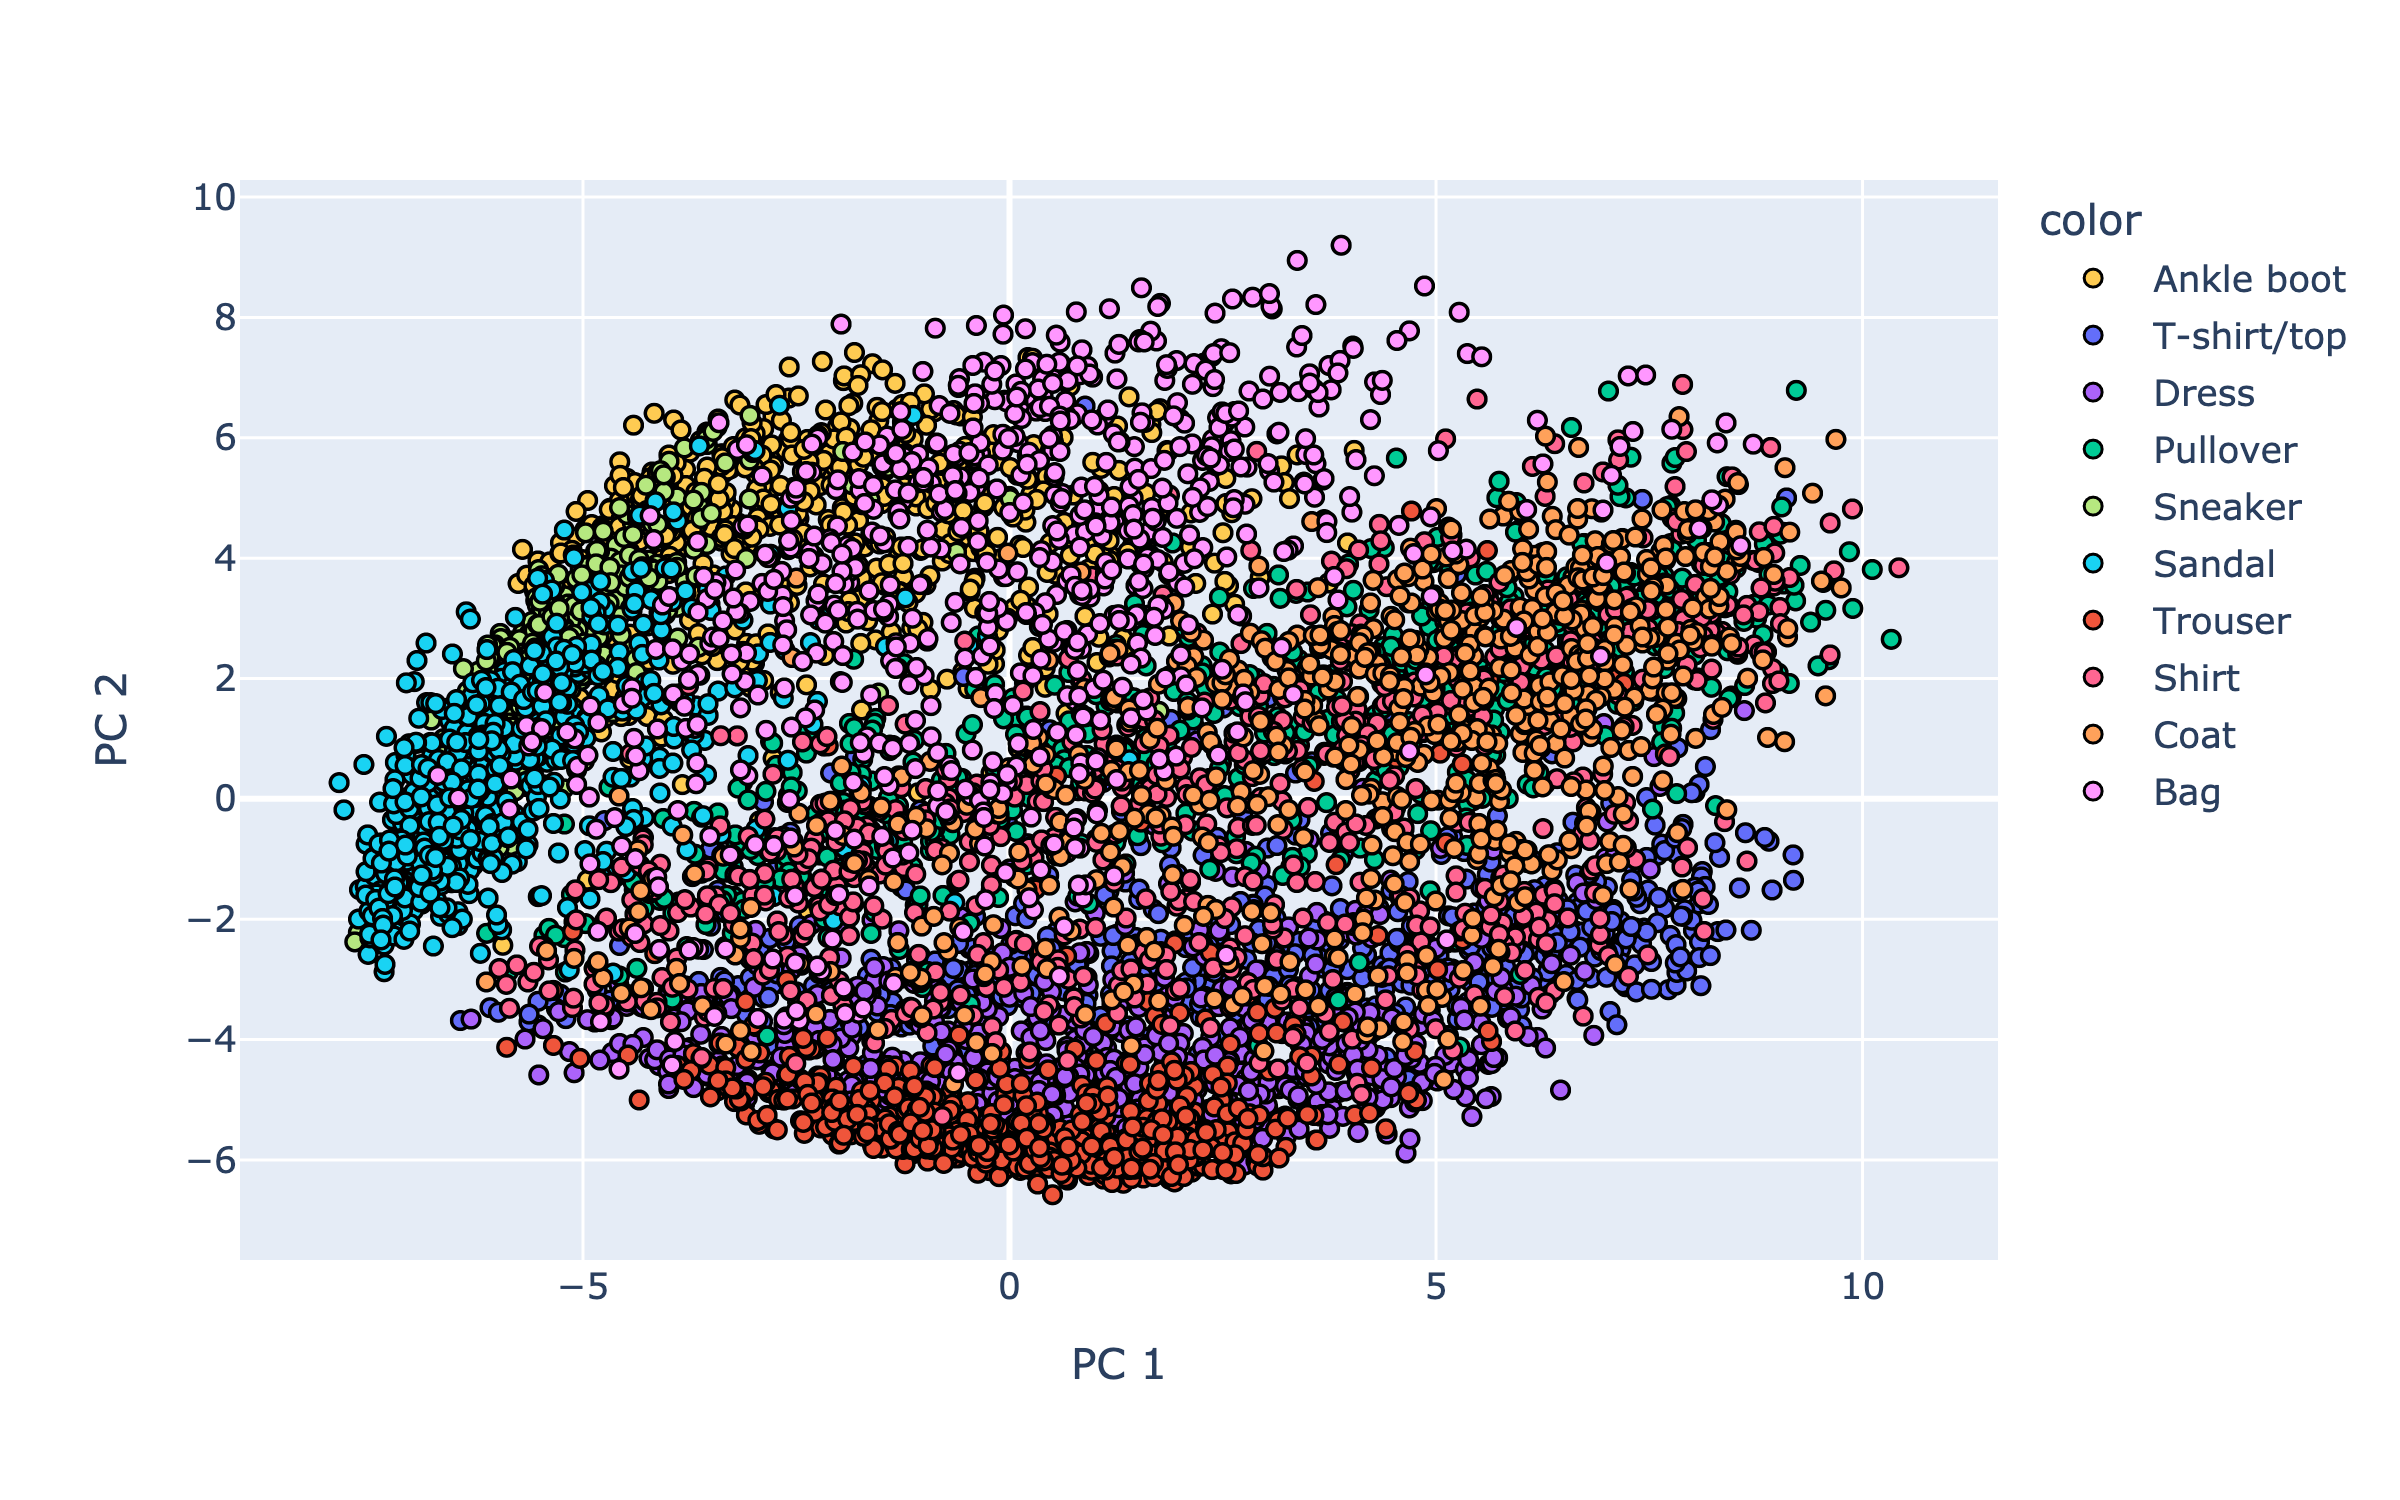
\includegraphics[width=1\linewidth]{images/PCA_2PC.png}
      \caption{\footnotesize Classic PCA, 2d projections }\label{Fig:PCA_2PC}
    \end{minipage}\hfill
    \begin{minipage}{0.5\textwidth}
      \centering
      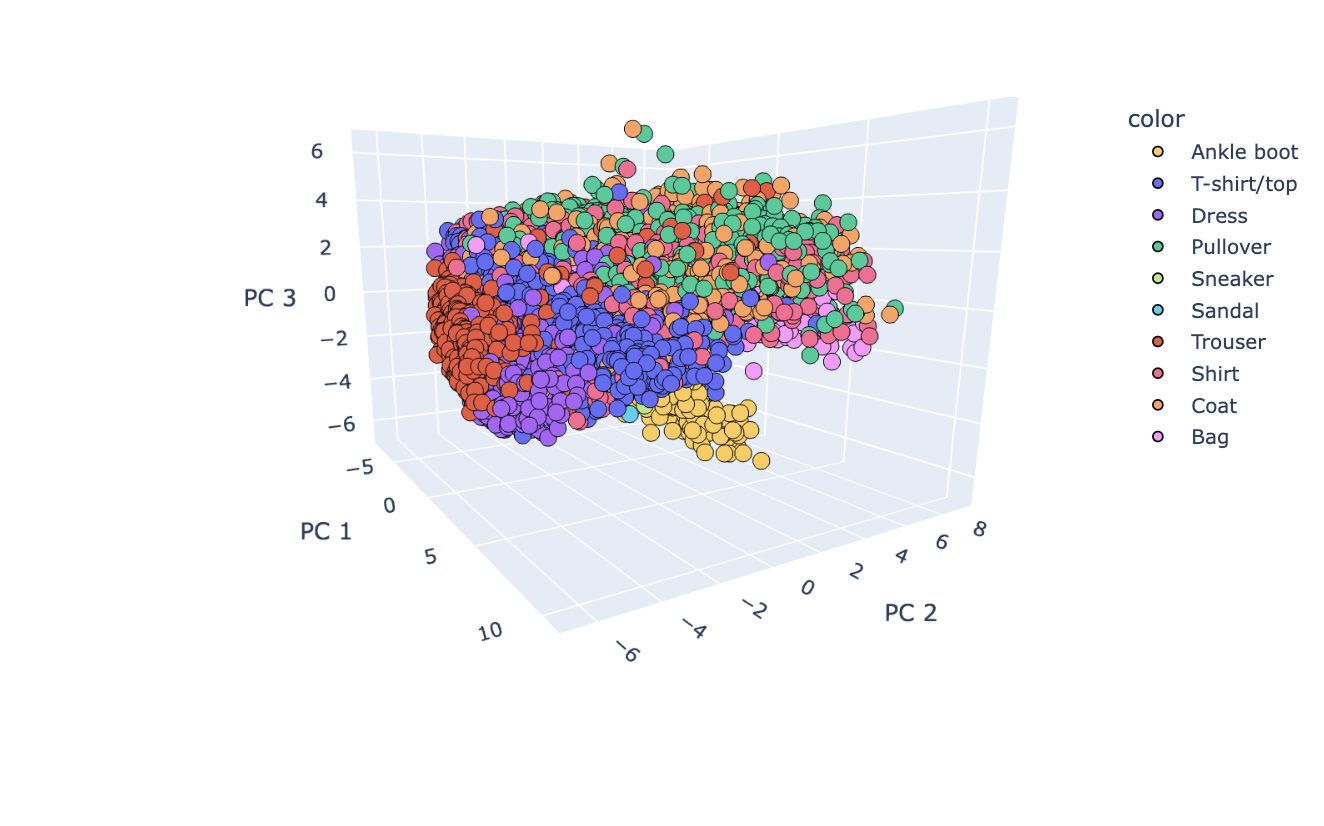
\includegraphics[width=1\linewidth]{images/PCA_3PC.png}
      \caption{\footnotesize Classic PCA, 3d projections}\label{Fig:PCA_3PC}
    \end{minipage}
 \end{figure}

 \begin{figure}[!htb]
    \begin{minipage}{0.5\textwidth}
      \centering
      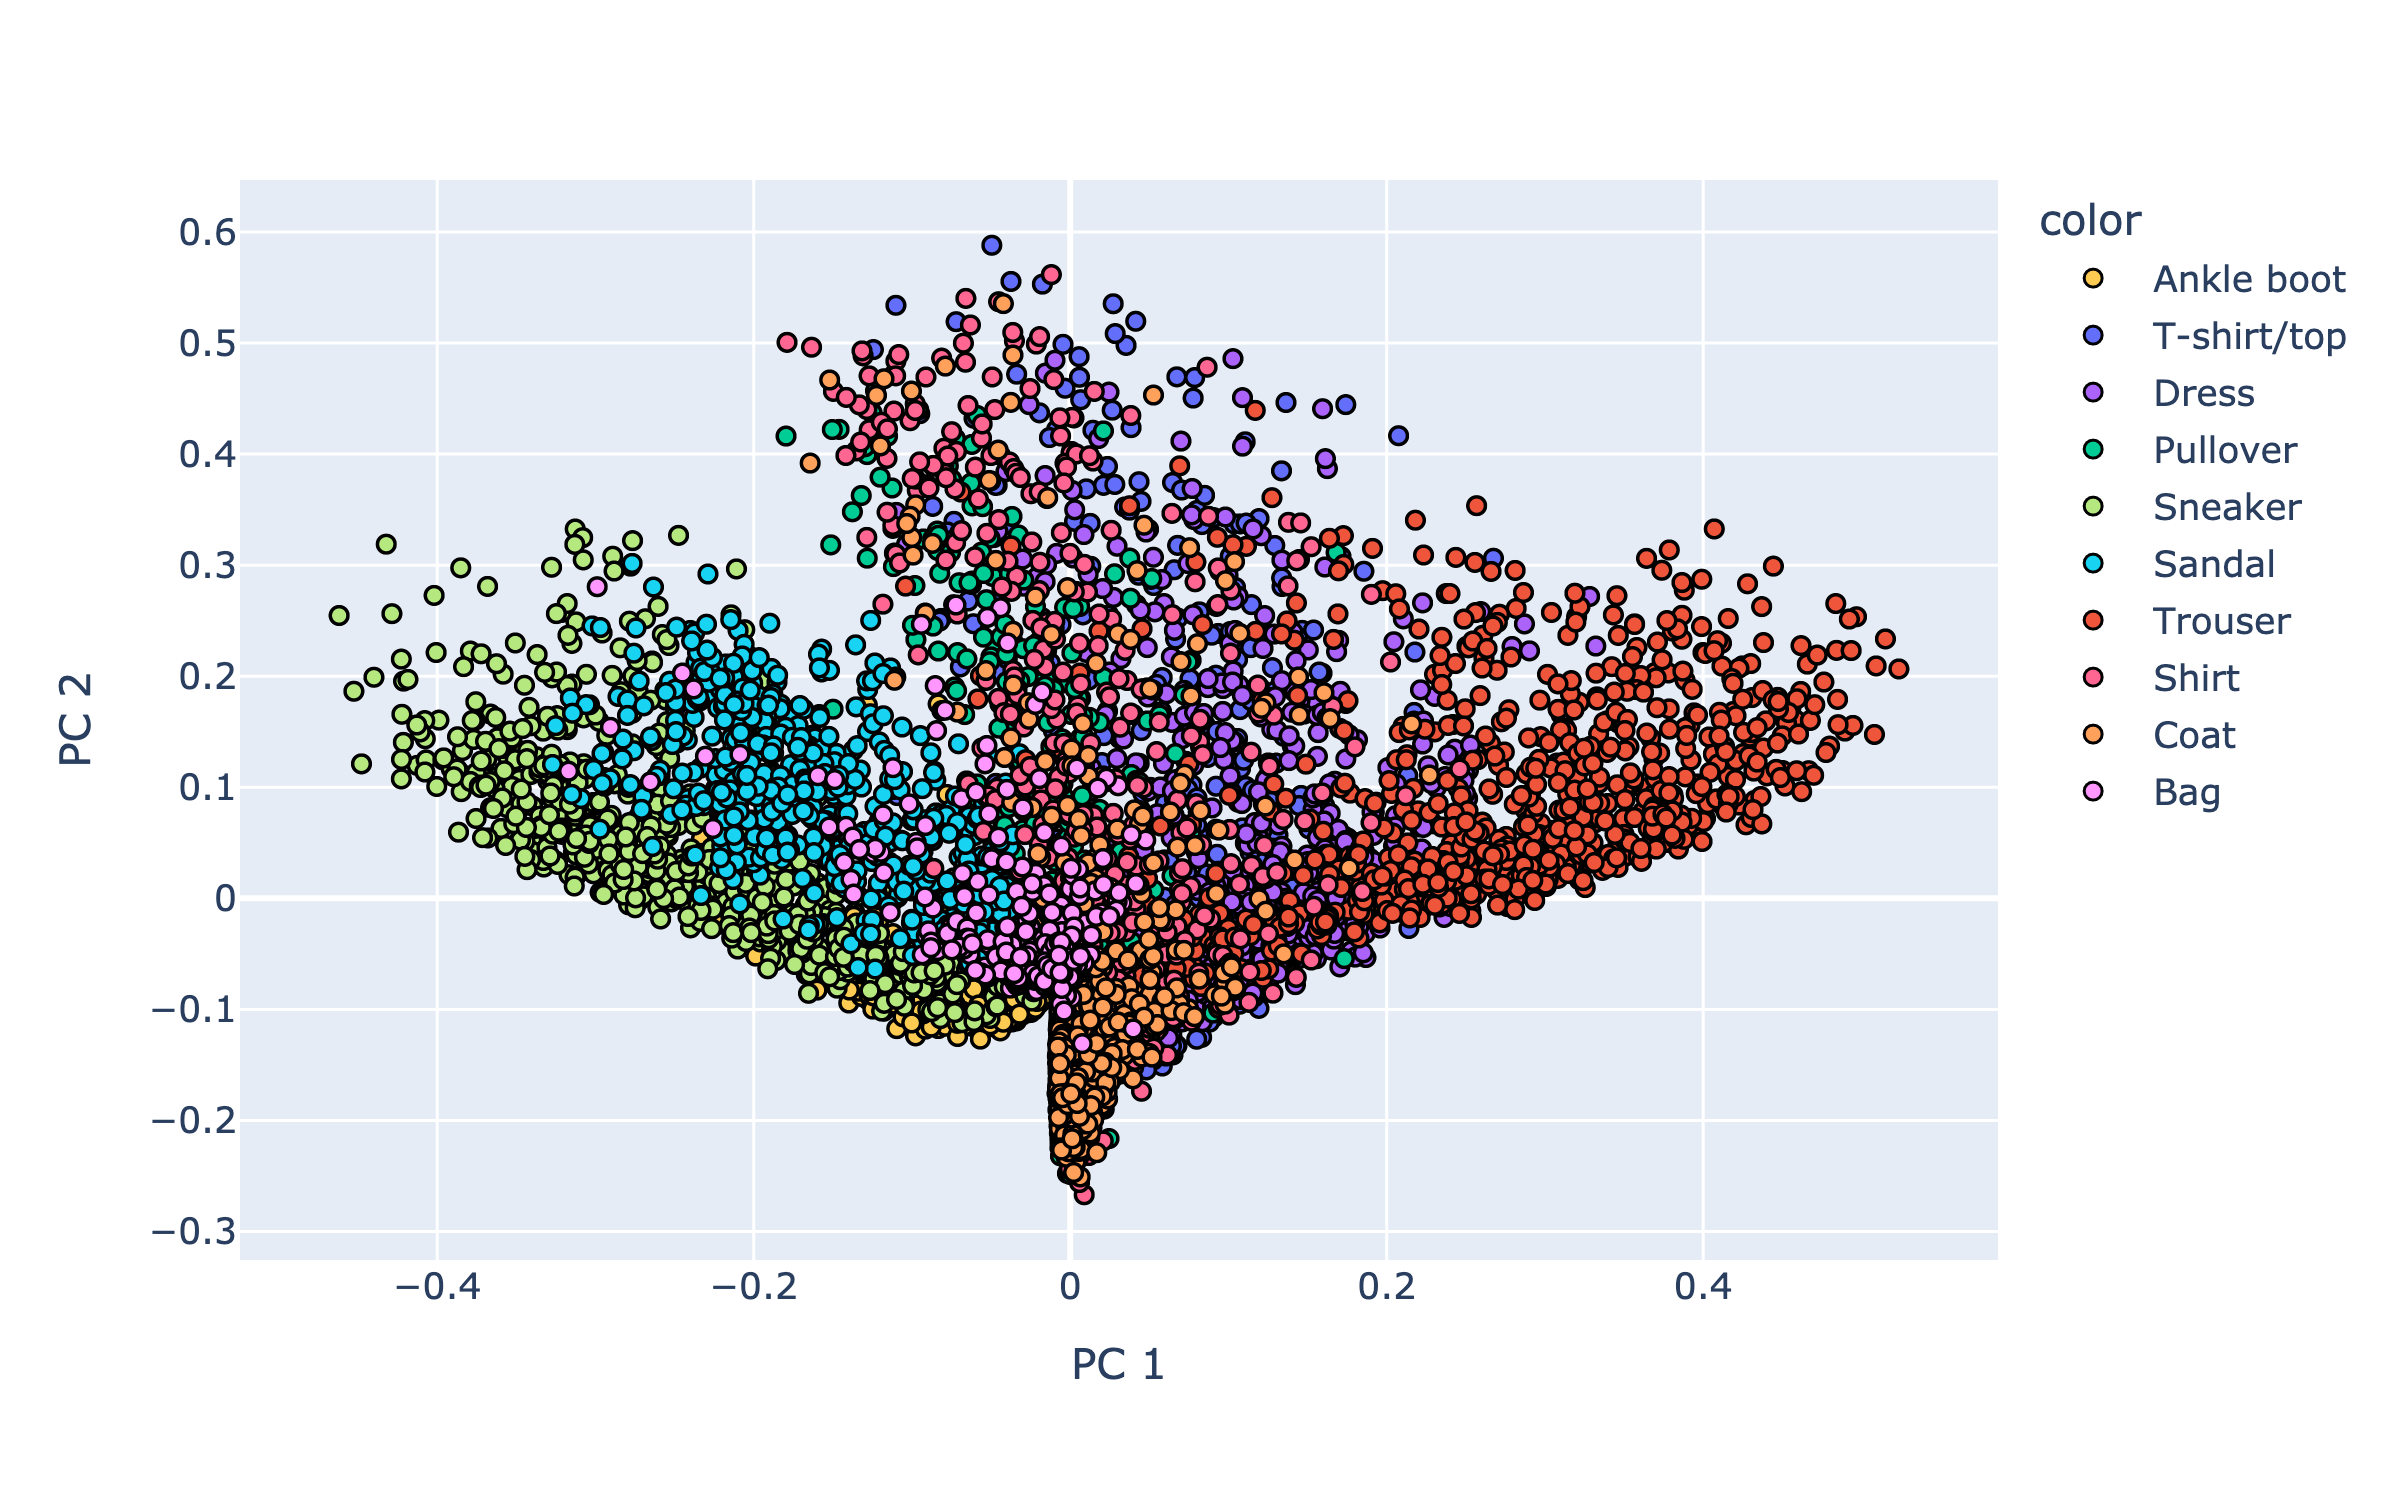
\includegraphics[width=1\linewidth]{images/rbfPCA_2PC.png}
      \caption{\footnotesize rbf kPCA ($\gamma=0.05$), 2d projections}\label{Fig:kPCA_2PC}
    \end{minipage}\hfill
    \begin{minipage}{0.5\textwidth}
      \centering
      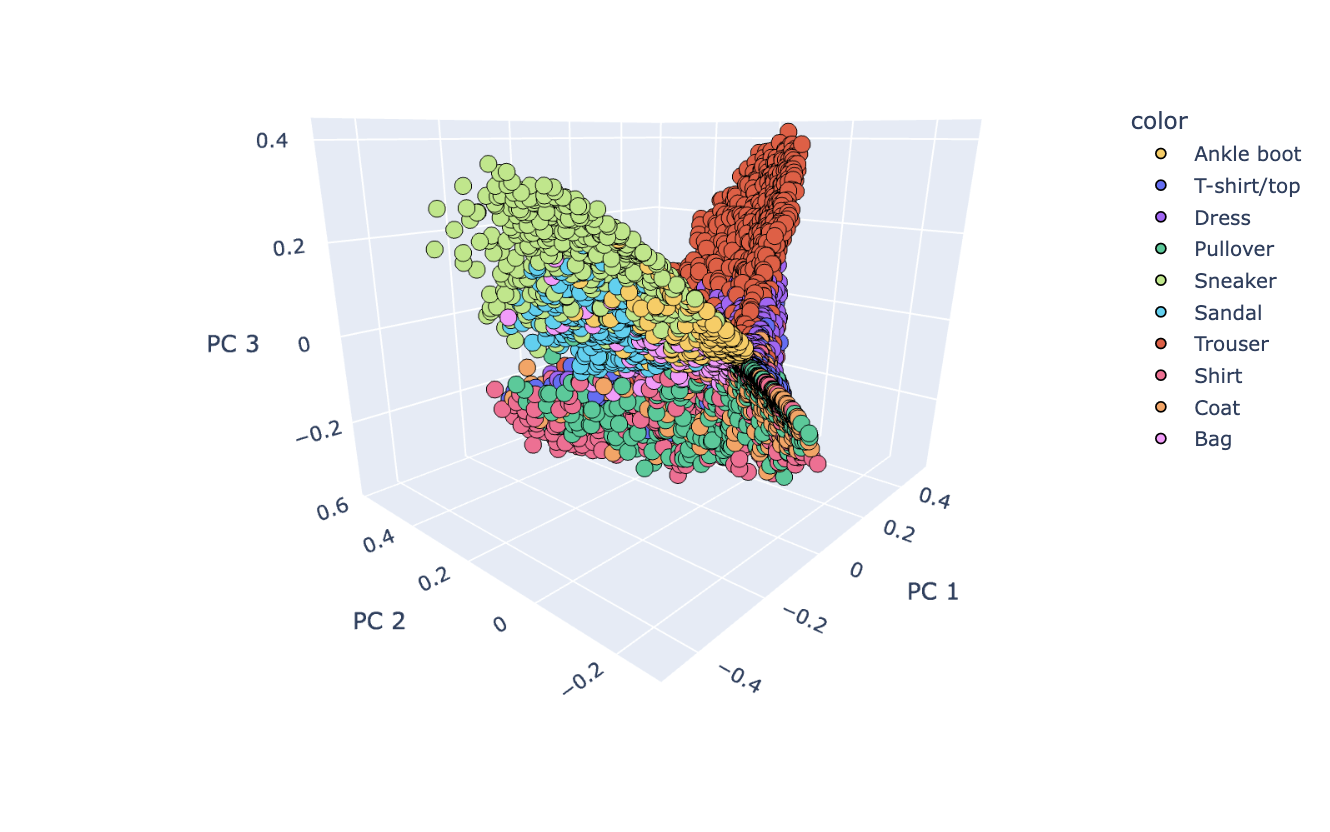
\includegraphics[width=1\linewidth]{images/rbfPCA_3PC.png}
      \caption{\footnotesize rbf kPCA ($\gamma=0.05$), 3d projections}\label{Fig:kPCA_3PC}
    \end{minipage}
 \end{figure}

Despite its simplicity, PCA managed to highlight some distinct groupings, as shown in \Cref{Fig:PCA_2PC,Fig:PCA_3PC}. Clear 
clusters are visible for categories such as bags, trousers, sandals, and ankle boots, with points in these groups appearing tightly concentrated. 
However, significant overlap remains among other classes, suggesting that PCA alone may not fully distinguish between all categories. I also 
experimented with polynomial PCA: a degree of 2 produced results similar to classical PCA, offering no notable improvement 
in cluster separation. Increasing the polynomial degree did not yield any substantial enhancement, either. Gaussian PCA, on the other hand, 
provided refined separation, especially for bags, trousers, sandals, and ankle boots, whose clusters appear even more distinctly defined. 
The dress category also shows improved separation, albeit less clearly in the plots. \Cref{Fig:kPCA_2PC,Fig:kPCA_3PC} reveal an 
interesting pattern: ankle boots, sandals, and sneakers form a cohesive region, while trousers are positioned more independently. This makes sense, 
given that ankle boots, sandals, and sneakers are all types of footwear, while trousers have features that set them apart from all the other labels 
in the dataset (if \emph{Fashion-MNIST} had included shorts or underwear, there might have been an overlapping with trousers).
Upper-body items like shirts, t-shirts, coats, and pullovers continue to overlap significantly, which is reasonable as they share 
similar shapes and visual traits.
%\newpage